\section{Discretizing the configuration space}
To apply quantum annealing to the deconflicting problem, we must encode the configuration space $\mathbf d$ in binary-valued variables.
To do so, we must first discretize and bound the allowed values.
Let $\Delta_d$ be the resolution of the allowed delays and $d_{\max} = N_d \Delta_d$ the maximum allowed delay, so that $d_i \in \left\{\Delta_d l \middle| l \in [0, 1, \ldots, N_d]\right\}$.
The larger the configuration space, the more qubits needed to encode it, and so determining the effect of this discretization on solution quality is integral to the effective use of quantum annealing.
To do so, we solve the deconflicting problem with departure delays only for various delay resolutions and upper bounds and compare the various optima to the continuous problem without restrictions (other than non-negativity) on the delays.
The exact optima are found by modeling the problem as a constraint satisfaction problem~\cite{numberjack}. 
We used as problem instances the non-trivially sized connected components of the conflict graph (as described in the previous section) for $d_{\max} = 18$; the largest such instance has $50$ flights and $104$ potential conflicts.

\begin{figure}[h]
\centering
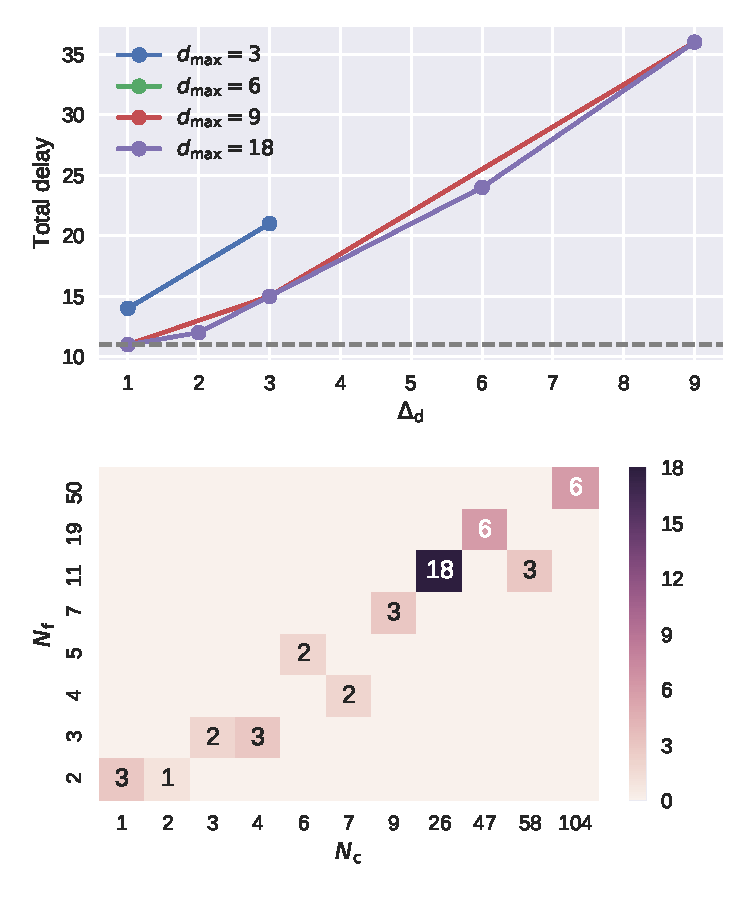
\includegraphics[width=0.45\textwidth]{./pics/delay_only_cp_results.pdf}
\caption[Effect of discretization on solution quality]{Top: Minimum total delay of a problem instance with $19$ flights and $47$ conflicts for various values of $\Delta_d$ and $d_{\max}$.
    Bottom: Minimum $d_\text{max}$ necessary to obtain same optimum as that without bounding the delay, for all non-trivial instances with $D_\text{max}=18$ and up to $50$ flights and $104$ conflicts.}
\label{fig:delay_only_cp_results}
\end{figure}

Figure~\ref{fig:delay_only_cp_results} shows the minimum total delay of a problem instance with $19$ flights and $47$ potential conflicts for various values of $\Delta_d$ and $d_{\max}$.
With the exception of the small maximum delay $d_\text{max} = 3$, the total delay of the solutions is nearly independent of the maximum delay.
The total delay is non-decreasing with respect to the coarseness $\Delta_d$ of the discretization for a fixed maximum delay $d_{\max}$, and non-increasing with respect to $d_{\max}$ for a fixed $\Delta_d$.
Since the original data is discretized in time in units of $1$ minute, $\Delta_d=1$ yield the same result as a continuous variable with the same upper bound.
Above some threshold value $d^0_\text{max}$, further increasing the maximum delay does not decrease the minimum total delay.
With one exception, we found that for all the investigated problem instances $d^0_\text{max}\leq6$ minutes (see Figure~\ref{fig:delay_only_cp_results}).
Therefore we conclude, that a moderate maximum delay is sufficient even for larger problem instances.
On the other hand, the delay discretization should be as fine as possible to obtain a high quality solutions.
